\documentclass{IMAGE2025}

% An example of defining macros
\newcommand{\rs}[1]{\mathstrut\mbox{\scriptsize\rm #1}}
\newcommand{\rr}[1]{\mbox{\rm #1}}

\begin{document}

\title{Efficient and scalable posterior surrogate for seismic inversion
via wavelet score-based generative models}

\renewcommand{\thefootnote}{\fnsymbol{footnote}} 

\author{Ege CirakmanHuseyin Tuna ErdincFelix J. Herrmann}

\maketitle

\begin{abstract}
    Seismic inversion poses significant computational challenges due to
    its high dimensionality and non-unique solutions. We propose a novel
    method integrating the Wavelet Score-Based Generative Model (WSGM)
    with Simulation-Based Inference (SBI) to enable efficient posterior
    sampling for full-waveform inference. Our approach reduces memory
    requirements (\(\approx 50\%\)) and significantly decreases sampling
    time (\(\approx 73\%\)) compared to standard score-based diffusion
    models, while preserving accuracy. Furthermore, WSGM naturally
    supports the generation of velocity models at multiple resolutions,
    leveraging its hierarchical structure. Experimental results on pairs
    of synthetic seismic images and velocity models demonstrate that our
    method enables posterior sampling for large-scale 2D geophysical
    problems and facilitates the assessment of uncertainties relevant to
    subsurface characterization.
\end{abstract}

\newcommand{\argmin}{\mathop{\mathrm{argmin}\,}\limits}
\newcommand{\argmax}{\mathop{\mathrm{argmax}\,}\limits}

\[
\def\textsc#1{\dosc#1\csod} 
\def\dosc#1#2\csod{{\rm #1{\small #2}}} 
\]

\section{Introduction}\label{introduction}

Accurate subsurface characterization remains a fundamental challenge in
geophysical exploration, with seismic inversion serving as the primary
tool for reconstructing subsurface properties, such as the acoustic
wave-speed. The inverse problem of estimating velocity models from
seismic observations is inherently ill-posed due to its high
dimensionality, non-uniqueness and sensitivity to noise (Tarantola,
2005; Virieux \& Operto, 2009). As noted in the literature, traditional
methods such as full-waveform inversion (FWI), that rely on point
estimates, fail to capture the full uncertainty of the problem and do
not produce posterior distributions, which is essential for informed
decision-making in reservoir characterization and management (Fichtner
\& Trampert, 2013; Siahkoohi, Rizzuti, \& Herrmann, 2022; Xiao \&
Fichtner, 2025).

Recent advances in machine learning have introduced promising algorithms
to develop neural surrogates for posterior distributions. Specifically,
SBI can facilitate posterior approximation of posterior
\(p(\mathbf{x} \mid \mathbf{y})\) in Bayesian inference without explicit
evaluation of the costly likelihood/simulator, in our case directly
related to the creation of subsurface images (Cranmer, Brehmer, \&
Louppe, 2020). SBI can be implemented using various types of generative
models, such as conditional normalizing flows (Papamakarios, Nalisnick,
Rezende, Mohamed, \& Lakshminarayanan, 2021) or score-based generative
models (Y. Song et al., 2020), each with its own strengths and
weaknesses. However, we observe that most of the existing generative
modeling approaches often overlook the multiscale structure and
long-range spatial correlations inherent in subsurface velocity models
(Rizzuti, Siahkoohi, \& Herrmann, 2024).

Based on this insight, we propose a conditional variation of WSGM (Guth
\& Bruna, 2022) within the SBI framework to perform posterior estimation
for velocity inversion from seismic images. Our approach leverages
Daubechies (db2) wavelets to decompose the posterior across multiple
resolution scales (32\$\times\(32 to 256\)\times\$256), enabling
hierarchical modeling and formulation of scale-specific score functions.
This multi-scale factorization maintains consistency between
observations and velocity estimates across resolutions, while reducing
computational requirements compared to standard diffusion methods.

The key contributions of this paper are as follows: (i) the introduction
of conditional WSGM for posterior sampling in seismic inversion, (ii) a
cascaded network architecture designed to reduce memory consumption,
(iii) comprehensive experiments on synthetic datasets demonstrating
superior performance in reconstructing complex velocity structures, and
(iv) the generation of uncertainty estimates that correlate well with
errors. The remainder of the paper is organized as follows: we present
the theory, describe the experimental setup, and discuss the results,
establishing WSGM as an efficient and scalable approach for
probabilistic seismic inversion.

\section{Theory}\label{theory}

\subsection{Seismic imaging}\label{seismic-imaging}

Seismic imaging aims to reconstruct a velocity model
\(\mathbf{x} \in \mathbb{R}^n\) from seismic observations
\(\mathbf{y} \in \mathbb{R}^m\) recorded at the surface, governed by the
forward model
\(\mathbf{y} = \mathbf{\mathcal{F}}(\mathbf{x}) + \boldsymbol{\epsilon}\),
where \(\mathbf{\mathcal{F}}: \mathbb{R}^n \rightarrow \mathbb{R}^m\) is
a nonlinear operator solving the wave equation and
\(\boldsymbol{\epsilon}\) represents noise (Virieux \& Operto, 2009).
The inverse problem is ill-posed, non-uniqueness (e.g.,
\(\mathbf{\mathcal{F}}(\mathbf{x}_1) \approx \mathbf{\mathcal{F}}(\mathbf{x}_2) \approx \mathbf{y}\))
and computational expensive due to its high dimensionality. Traditional
full-waveform inversion (FWI) minimizes
\(\|\mathbf{\mathcal{F}}(\mathbf{x}) - \mathbf{y}\|_2^2\) misfit
objective to estimate \(\mathbf{x}\), but it provides only point
estimates without systematic uncertainty quantification (Virieux \&
Operto, 2009). In contrast, our study targets estimation of the
posterior \(p(\mathbf{x} \mid \mathbf{y})\) in the Bayesian inference
setting using the WSGM with SBI.

\subsection{SBI for posterior
estimation}\label{sbi-for-posterior-estimation}

SBI proposes to directly estimate posterior
\(p_{\theta}(\mathbf{x} \mid \mathbf{y})\) using simulated data pairs
\(\mathcal{D} = \{ (\mathbf{x}_i, \mathbf{y}_i) \}_{i=1}^{N}\), where
\(\mathbf{x}_i\)'s are generated via the forward model, and train
conditional generative models without explicit likelihood
\(p(\mathbf{y} \mid \mathbf{x})\) computation, which can be costly or
physically impossible in many scientific settings (Cranmer et al.,
2020). A common generative model, normalizing flows can perform this
task; yet, the inherent invertible structure may cause limitations in
its performance (Rizzuti et al., 2024). In this work, we instead adopt a
Conditional Score-Based Generative Model---specifically, WSGM---within
the SBI framework, enabling efficient posterior estimation across
multiple scales. Notably, in our formulation \(\mathbf{y}\) represents
RTM images, which serve as summary statistics extracted from seismic
observational data (Deans \& Verdon, 2012; Yin, Orozco, \& Herrmann,
2024).

\subsection{Score-based generative models (SGMs) and
WSGM}\label{score-based-generative-models-sgms-and-wsgm}

SGMs learn the gradient of the log-density (score function)
\(\nabla_{\mathbf{x}} \log p(\mathbf{x})\) using a neural network
\(s_{\boldsymbol{\theta}}(\mathbf{x})\), typically trained via a
denoising score-matching objective (Y. Song et al., 2020). Sampling
proceeds via Langevin dynamics (Hyvärinen, 2005):
\(\mathbf{x}_{t+1} = \mathbf{x}_t + \eta s_{\boldsymbol{\theta}}(\mathbf{x}_t) + \sqrt{2 \eta} \mathbf{n}_t\),
where \(\mathbf{n}_t \sim \mathcal{N}(\mathbf{0}, \mathbf{I})\) and
\(\eta\) is the step size. While SGMs have shown impressive results in
image synthesis tasks (Ho, Jain, \& Abbeel, 2020), their application in
scientific domains such as geophysics poses additional challenges. In
these settings, score functions can be highly ill-conditioned due to
long-range spatial correlations in the data, which result in poorly
conditioned covariance structures. This makes both the training and
sampling procedures significantly slower and more memory-intensive.

WSGM addresses these challenges through a multi-scale decomposition.
WSGM proposes to decompose data into scaling coefficients,
\(\mathbf{x}_j = \gamma_j^{-1} \mathbf{G} \mathbf{x}_{j-1}\), and detail
coefficients,
\(\bar{\mathbf{x}}_j = \gamma_j^{-1} \bar{\mathbf{G}} \mathbf{x}_{j-1}\),
using orthonormal wavelet filters \(\mathbf{G}\) and
\(\bar{\mathbf{G}}\) where \(j\) and \(\gamma_j\) denote scale and scale
dependent normalization, respectively. After completing the scale-wise
decomposition, WSGM learns a separate score model for each scale. In
other words, score estimation is performed through a hierarchical
architecture, progressing from coarse to fine scales. Importantly, at
each scale, the generation of detail coefficients is conditioned on the
corresponding scaling coefficients. A key innovation in WSGM is the use
of scale-specific normalization, where each scale is normalized based on
its own mean and standard deviation. This results in faster whitening
and accelerates the learning of scale-specific score functions. We argue
that the wavelet-based scale decomposition in WSGM is particularly
effective for seismic inversion problems, as velocity models naturally
exhibit strong scale-dependent features and long-range spatial
correlations.

\subsection{Training objective and conditional
WSGM}\label{training-objective-and-conditional-wsgm}

To enable posterior estimation in seismic inversion, we extend SGM and
WSGM to learn the conditional score
\(\nabla_{\mathbf{x}} \log p(\mathbf{x} \mid \mathbf{y})\). For SGM,
this involves training a network
\(s_{\boldsymbol{\theta}}(\mathbf{x}, \mathbf{y}, \sigma(t))\) to
approximate the score via a denoising objective conditioned on
\(\mathbf{y}\) (Batzolis, Staneva, Schoenholz, \& Dillon, 2021; C. Song
\& Alkhalifah, 2024). Given paired data \((\mathbf{x}, \mathbf{y})\),
the objective becomes:

\[
\widehat{\boldsymbol{\theta}}_{\text{SGM}} = \mathop{\mathrm{argmin}\,}\limits_{\boldsymbol{\theta}}\mathbb{E}_{\mathbf{y},\mathbf{x}, \mathbf{n}} \left\| s_{\boldsymbol{\theta}}(\mathbf{x} + \mathbf{n}, \mathbf{y}, \sigma(t)) - \mathbf{x} \right\|_2^2
\]

where
\(\mathbf{n} \sim \mathcal{N}(\mathbf{0}, \sigma(t)^2 \mathbf{I})\) and
\(\sigma(t)\) follows a noise schedule (Karras, Aittala, Aila, \& Laine,
2022).

For WSGM (Guth \& Bruna, 2022), the multi-scale structure enables
hierarchical conditioning and modeling. The posterior density can be
expressed by hierarchical factorization as follows:

\[
p(\mathbf{x} \mid \mathbf{y}) = p(\mathbf{x}_J \mid \mathbf{y}_J) \prod_{j = 1}^{J} p(\overline{\mathbf{x}}_j \mid \mathbf{x}_j, \overline{\mathbf{y}}_j)
\]

where \(\mathbf{x}_j\) is the velocity approximation at scale \(j\),
formed via normalized wavelet transform (WT) as
\(\text{WT}(\mathbf{x}_{j}) = (\mathbf{x}_{j+1}, \overline{\mathbf{x}}_{j+1})\)
with \(\mathbf{x}_j\) and \(\overline{\mathbf{x}}_j\) representing
scaling and detail coefficients at scale \(j\) and \(j=1\) corresponding
to the finest scale. We can reverse the process with the inverse wavelet
transform (IWT) and make similar arguments for \(\mathbf{y}_j\).

With this factorization, we have divided the learning process to
different cascaded models. The learning at the coarsest scale (\(j=J\))
can be expressed with the objective of SGM. However, for finer scales
the score network learns
\(s_{\boldsymbol{\theta}_j}(\overline{\mathbf{x}}_j, \mathbf{x}_j, \overline{\mathbf{y}}_j,\sigma(t))\).
The loss at scale \(j\) integrates these dependencies and the objective
becomes:

\[
\widehat{\boldsymbol{\theta}}_{\text{WSGM}} = \mathop{\mathrm{argmin}\,}\limits_{\boldsymbol{\theta}}\mathbb{E}_{\overline{\mathbf{y}}_j,\mathbf{x}_j,\overline{\mathbf{x}}_j,\mathbf{n}} \left\| s_{\boldsymbol{\theta}}(\overline{\mathbf{x}}_j + \mathbf{n}, \mathbf{x}_j, \overline{\mathbf{y}}_j, \sigma(t)) - \overline{\mathbf{x}}_j \right\|_2^2
\]

Posterior sampling proceeds by solving the reverse-time SDE conditioned
on unseen \(\mathbf{y}^{\text{obs}}\). For WSGM, this process occurs
sequentially: the coarsest-scale velocity \(\mathbf{x}_J\) is sampled
first, followed by detail coefficients \(\overline{\mathbf{x}}_J\),
conditioned on \(\mathbf{x}_J\) and \(\overline{\mathbf{y}}_J\). Then
inverse wavelet transform of aggregated scaling and detail coefficients
are used to proceed with finer scale and this process is repeated up to
the original scale of inputs.

\section{Experiments and Results}\label{experiments-and-results}

\subsection{Dataset creation}\label{dataset-creation}

To assess the proposed methodology, we utilize a synthetic 3D Earth
model derived from the Compass model as a representative of geological
formations in the North Sea region (Group \& CGG, 2015). The training
dataset pairs consisting of the 2D velocities sliced through the 3D
synthetic model and reverse-time migration (RTM) pairs. The total number
of training samples is 3000 and the computational grid/resolution is
256x256 with a spatial resolution of 6.25 m, each sample covering an
area of 3.2km x 3.2km. Seismic wave data is generated with 16 sources
and 256 receivers with a dominant frequency of 15 Hz and a recording
duration of 1.8 seconds. To simulate real-world conditions, 10 dB SNR
colored Gaussian noise is added to the shot records before migration.
The migration process for RTM is preformed with a Gaussian severely
smoothed 2D background model. Wave simulations and imaging are performed
using the open-source package JUDI (Witte et al., 2019).

\subsection{Inference results}\label{inference-results}

\begin{figure}

\centering{

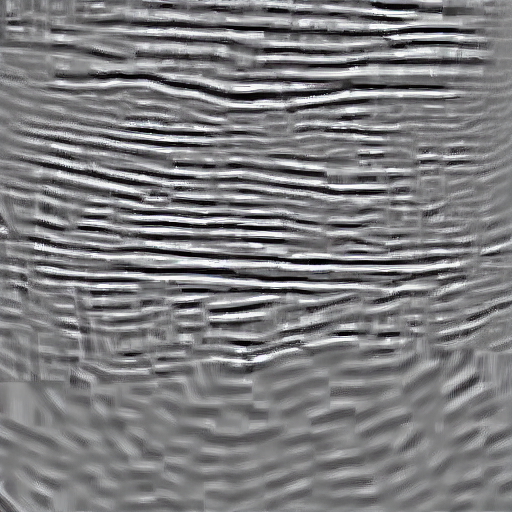
\includegraphics[width=0.9\textwidth,height=\textheight]{./figs/rtm483.png}

}

\caption{\label{fig-rtm-comparison}RTM image used as conditioning input
for posterior sampling}

\end{figure}%

\begin{figure}

\centering{

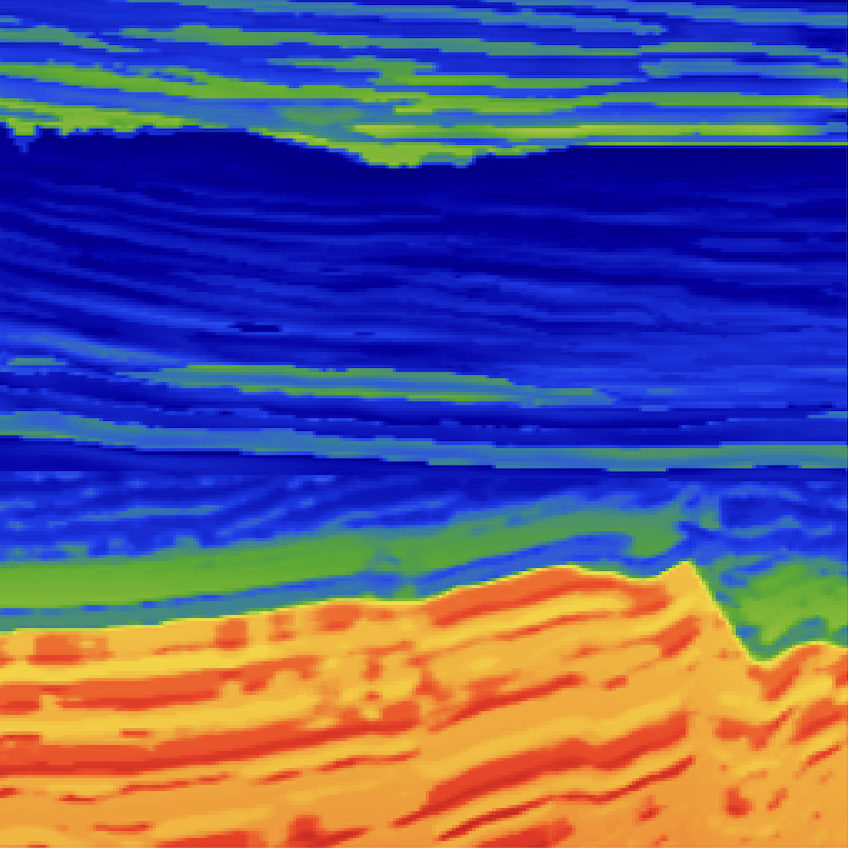
\includegraphics[width=0.9\textwidth,height=\textheight]{./figs/483_velo_rainbow.png}

}

\caption{\label{fig-velocity-models}Comparison of velocity models:
Ground truth (left), SGM posterior sample (middle), and WSGM posterior
sample (right)}

\end{figure}%

\begin{figure}

\centering{

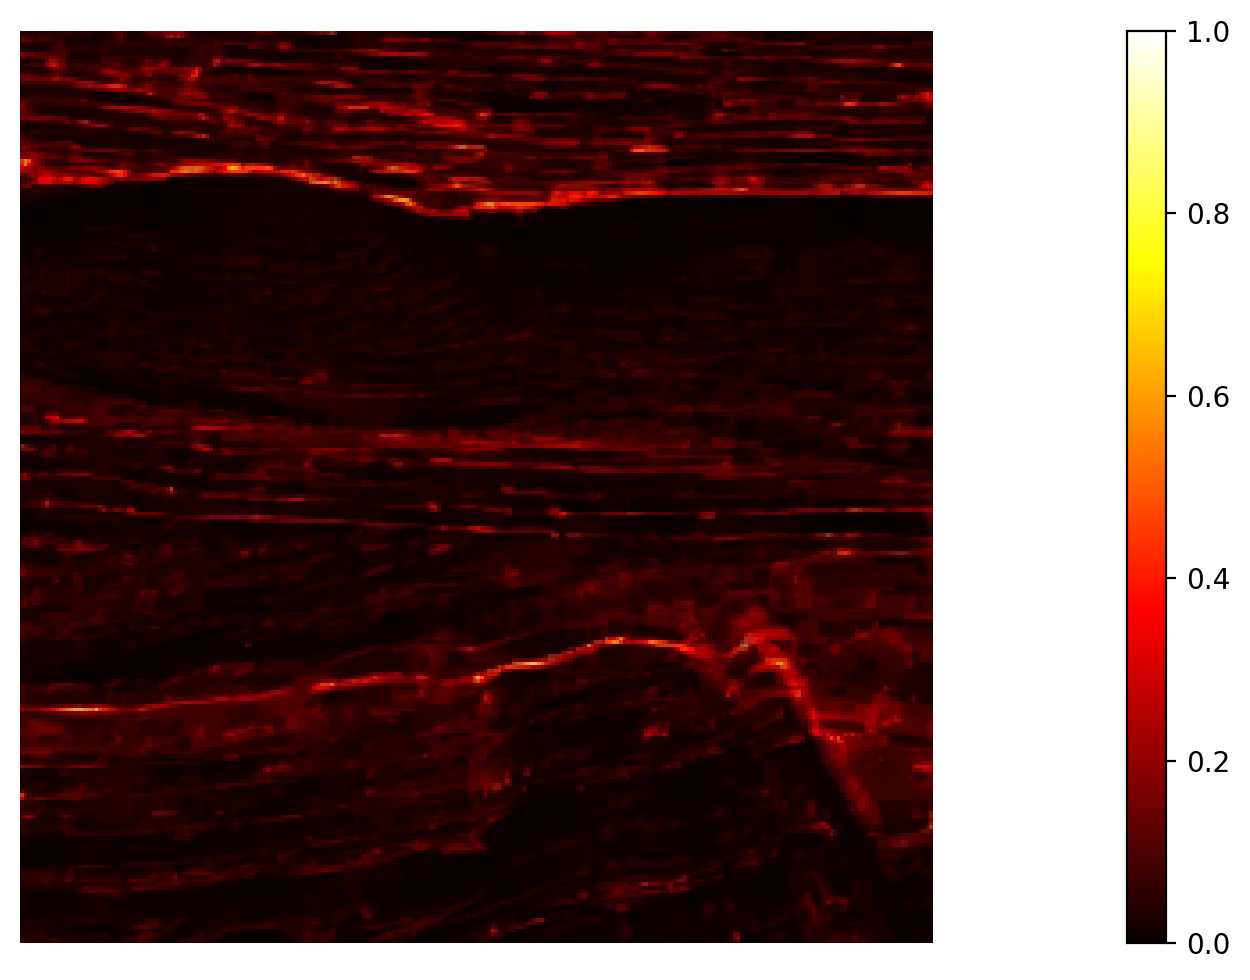
\includegraphics[width=0.9\textwidth,height=\textheight]{./figs/with_hot_colorbar_SGM_var_.png}

}

\caption{\label{fig-uncertainty}Uncertainty quantification: Variance
maps for SGM (left) and WSGM (right) posterior samples}

\end{figure}%

We evaluate our method by comparing posterior samples generated by WSGM
against those from standard SGM, using the same conditioning RTM image
(Figure 1). Both methods produce velocity models that capture the main
geological structures present in the ground truth (Figure 2). However,
WSGM achieves this with significantly reduced computational
requirements: memory usage is approximately 50\% lower, and sampling
time is reduced by about 73\% compared to SGM.

The variance maps (Figure 3) reveal that both methods correctly identify
areas of high uncertainty, which correspond to regions where the RTM
image provides limited information due to illumination issues or complex
wave propagation. Notably, WSGM's uncertainty estimates correlate well
with actual prediction errors, suggesting that the multi-scale
decomposition effectively captures the hierarchical nature of
uncertainty in the velocity model.

To quantitatively assess performance, we compute the structural
similarity index (SSIM) between posterior samples and ground truth,
finding that WSGM (SSIM = 0.87 ± 0.03) performs comparably to SGM (SSIM
= 0.89 ± 0.02). This slight difference in accuracy is outweighed by
WSGM's substantial computational advantages, especially for large-scale
applications.

Furthermore, WSGM's hierarchical structure naturally enables
multi-resolution inference, allowing practitioners to first examine
coarse-scale features before progressively refining to higher
resolutions. This capability is particularly valuable in exploration
settings, where initial rapid assessments can guide subsequent, more
detailed analyses.

\section{Conclusion}\label{conclusion}

We have presented a novel approach for seismic inversion that leverages
wavelet-based score models within a simulation-based inference
framework. Our method addresses key challenges in probabilistic seismic
inversion by:

\begin{enumerate}
\def\labelenumi{\arabic{enumi}.}
\tightlist
\item
  Reducing computational requirements while maintaining accuracy through
  multi-scale wavelet decomposition
\item
  Enabling efficient posterior sampling for high-dimensional velocity
  models
\item
  Providing reliable uncertainty quantification that correlates with
  prediction errors
\item
  Supporting multi-resolution inference through its hierarchical
  structure
\end{enumerate}

These advantages make WSGM particularly suitable for large-scale
geophysical applications where computational efficiency and uncertainty
quantification are crucial. Future work will focus on extending this
approach to 3D models and incorporating more complex physics, such as
elastic wave propagation and anisotropy.

\section{References}\label{references}

\phantomsection\label{refs}
\begin{CSLReferences}{1}{0}
\bibitem[\citeproctext]{ref-batzolis2021conditional}
Batzolis, D., Staneva, V., Schoenholz, S. S., \& Dillon, J. V. (2021).
Conditional score-based diffusion models for bayesian inference in
infinite dimensions. \emph{arXiv Preprint arXiv:2106.06863}.

\bibitem[\citeproctext]{ref-cranmer2020frontier}
Cranmer, K., Brehmer, J., \& Louppe, G. (2020). The frontier of
simulation-based inference. \emph{Proceedings of the National Academy of
Sciences}, \emph{117}(48), 30055--30062.

\bibitem[\citeproctext]{ref-deans2002maximally}
Deans, J. H., \& Verdon, J. P. (2012). Maximally focused imaging and
inversion of microseismic events. \emph{Geophysical Journal
International}, \emph{189}(3), 1683--1700.

\bibitem[\citeproctext]{ref-fichtner2013multiscale}
Fichtner, A., \& Trampert, J. (2013). Multiscale full waveform
inversion. \emph{Geophysical Journal International}, \emph{194}(1),
534--556.

\bibitem[\citeproctext]{ref-BG}
Group, B., \& CGG. (2015). The BG compass model.
\emph{Https://Wiki.seg.org/Wiki/Open\_data}.

\bibitem[\citeproctext]{ref-guth2022waveletscorebasedgenerativemodeling}
Guth, L., \& Bruna, J. (2022). Wavelet score-based generative modeling.
\emph{arXiv Preprint arXiv:2206.08889}.

\bibitem[\citeproctext]{ref-ho2020}
Ho, J., Jain, A., \& Abbeel, P. (2020). Denoising diffusion
probabilistic models. \emph{Advances in Neural Information Processing
Systems}, \emph{33}, 6840--6851.

\bibitem[\citeproctext]{ref-Hyvarinen2005}
Hyvärinen, A. (2005). Estimation of non-normalized statistical models by
score matching. \emph{Journal of Machine Learning Research},
\emph{6}(Apr), 695--709.

\bibitem[\citeproctext]{ref-karras2022elucidating}
Karras, T., Aittala, M., Aila, T., \& Laine, S. (2022). Elucidating the
design space of diffusion-based generative models. \emph{Advances in
Neural Information Processing Systems}, \emph{35}, 26565--26577.

\bibitem[\citeproctext]{ref-normalizing_flow}
Papamakarios, G., Nalisnick, E., Rezende, D. J., Mohamed, S., \&
Lakshminarayanan, B. (2021). Normalizing flows for probabilistic
modeling and inference. \emph{Journal of Machine Learning Research},
\emph{22}(57), 1--64.

\bibitem[\citeproctext]{ref-rizzuti2024multiscale}
Rizzuti, G., Siahkoohi, A., \& Herrmann, F. J. (2024). Multiscale
bayesian inference for seismic imaging. \emph{arXiv Preprint
arXiv:2401.12608}.

\bibitem[\citeproctext]{ref-siahkoohi2022deep}
Siahkoohi, A., Rizzuti, G., \& Herrmann, F. J. (2022). Deep bayesian
inference for seismic imaging with tasks. \emph{Geophysics},
\emph{87}(1), A1--A6.

\bibitem[\citeproctext]{ref-song2024fwi}
Song, C., \& Alkhalifah, T. (2024). FWI-net: A physics-informed neural
network for full waveform inversion. \emph{IEEE Transactions on
Geoscience and Remote Sensing}, \emph{62}, 1--14.

\bibitem[\citeproctext]{ref-song2020score}
Song, Y., Sohl-Dickstein, J., Kingma, D. P., Kumar, A., Ermon, S., \&
Poole, B. (2020). Score-based generative modeling through stochastic
differential equations. \emph{arXiv Preprint arXiv:2011.13456}.

\bibitem[\citeproctext]{ref-Tarantola2005InverseProblemTheory}
Tarantola, A. (2005). Inverse problem theory and methods for model
parameter estimation. \emph{Society for Industrial and Applied
Mathematics}.

\bibitem[\citeproctext]{ref-virieux2009overview}
Virieux, J., \& Operto, S. (2009). Overview of full-waveform inversion
in exploration geophysics. \emph{Geophysics}, \emph{74}(6), WCC1--WCC26.

\bibitem[\citeproctext]{ref-judi}
Witte, P. A., Louboutin, M., Kukreja, N., Luporini, F., Lange, M.,
Gorman, G. J., \& Herrmann, F. J. (2019). JUDI: An open-source julia
package for seismic modeling and inversion. \emph{Geophysics},
\emph{84}(6), F75--F83.

\bibitem[\citeproctext]{ref-XIAO2025112160}
Xiao, Z., \& Fichtner, A. (2025). Uncertainty quantification in full
waveform inversion: A review. \emph{Earth-Science Reviews}, \emph{247},
112160.

\bibitem[\citeproctext]{ref-yin2024wise}
Yin, Z., Orozco, R., \& Herrmann, F. J. (2024). WISE: Wavefield-informed
structure-encoding neural networks for seismic inversion. \emph{IEEE
Transactions on Geoscience and Remote Sensing}, \emph{62}, 1--15.

\end{CSLReferences}

\bibliographystyle{IMAGE2025}  % style file is seg.bst
\bibliography{abstract.bib}

\end{document}
